% Created by tikzDevice version 0.10.1 on 2016-08-19 15:28:36
% !TEX encoding = UTF-8 Unicode
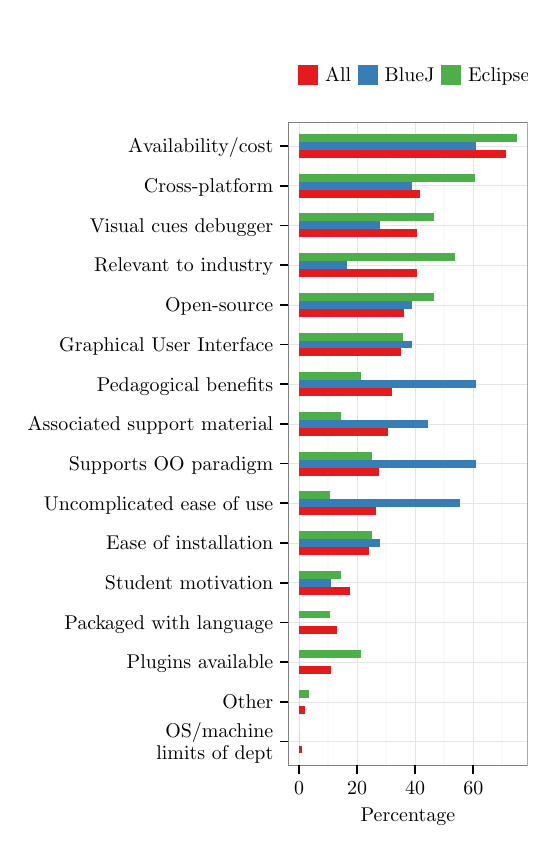
\begin{tikzpicture}[x=1pt,y=1pt]
\definecolor{fillColor}{RGB}{255,255,255}
\path[use as bounding box,fill=fillColor,fill opacity=0.00] (0,0) rectangle (180.67,289.08);
\begin{scope}
\path[clip] (  0.00,  0.00) rectangle (180.67,289.08);
\definecolor{drawColor}{RGB}{255,255,255}
\definecolor{fillColor}{RGB}{255,255,255}

\path[draw=drawColor,line width= 0.6pt,line join=round,line cap=round,fill=fillColor] (  0.00,  0.00) rectangle (180.68,289.08);
\end{scope}
\begin{scope}
\path[clip] ( 94.14, 22.52) rectangle (180.67,254.94);
\definecolor{fillColor}{RGB}{255,255,255}

\path[fill=fillColor] ( 94.14, 22.52) rectangle (180.67,254.94);
\definecolor{drawColor}{gray}{0.98}

\path[draw=drawColor,line width= 0.6pt,line join=round] (108.56, 22.52) --
	(108.56,254.94);

\path[draw=drawColor,line width= 0.6pt,line join=round] (129.54, 22.52) --
	(129.54,254.94);

\path[draw=drawColor,line width= 0.6pt,line join=round] (150.52, 22.52) --
	(150.52,254.94);

\path[draw=drawColor,line width= 0.6pt,line join=round] (171.50, 22.52) --
	(171.50,254.94);
\definecolor{drawColor}{gray}{0.90}

\path[draw=drawColor,line width= 0.2pt,line join=round] ( 94.14, 31.13) --
	(180.67, 31.13);

\path[draw=drawColor,line width= 0.2pt,line join=round] ( 94.14, 45.47) --
	(180.67, 45.47);

\path[draw=drawColor,line width= 0.2pt,line join=round] ( 94.14, 59.82) --
	(180.67, 59.82);

\path[draw=drawColor,line width= 0.2pt,line join=round] ( 94.14, 74.17) --
	(180.67, 74.17);

\path[draw=drawColor,line width= 0.2pt,line join=round] ( 94.14, 88.51) --
	(180.67, 88.51);

\path[draw=drawColor,line width= 0.2pt,line join=round] ( 94.14,102.86) --
	(180.67,102.86);

\path[draw=drawColor,line width= 0.2pt,line join=round] ( 94.14,117.21) --
	(180.67,117.21);

\path[draw=drawColor,line width= 0.2pt,line join=round] ( 94.14,131.55) --
	(180.67,131.55);

\path[draw=drawColor,line width= 0.2pt,line join=round] ( 94.14,145.90) --
	(180.67,145.90);

\path[draw=drawColor,line width= 0.2pt,line join=round] ( 94.14,160.25) --
	(180.67,160.25);

\path[draw=drawColor,line width= 0.2pt,line join=round] ( 94.14,174.59) --
	(180.67,174.59);

\path[draw=drawColor,line width= 0.2pt,line join=round] ( 94.14,188.94) --
	(180.67,188.94);

\path[draw=drawColor,line width= 0.2pt,line join=round] ( 94.14,203.29) --
	(180.67,203.29);

\path[draw=drawColor,line width= 0.2pt,line join=round] ( 94.14,217.63) --
	(180.67,217.63);

\path[draw=drawColor,line width= 0.2pt,line join=round] ( 94.14,231.98) --
	(180.67,231.98);

\path[draw=drawColor,line width= 0.2pt,line join=round] ( 94.14,246.33) --
	(180.67,246.33);

\path[draw=drawColor,line width= 0.2pt,line join=round] ( 98.07, 22.52) --
	( 98.07,254.94);

\path[draw=drawColor,line width= 0.2pt,line join=round] (119.05, 22.52) --
	(119.05,254.94);

\path[draw=drawColor,line width= 0.2pt,line join=round] (140.03, 22.52) --
	(140.03,254.94);

\path[draw=drawColor,line width= 0.2pt,line join=round] (161.01, 22.52) --
	(161.01,254.94);
\definecolor{fillColor}{RGB}{228,26,28}

\path[fill=fillColor] ( 98.07, 26.82) rectangle ( 99.23, 29.69);
\definecolor{fillColor}{RGB}{77,175,74}

\path[fill=fillColor] ( 98.07, 32.56) rectangle ( 98.07, 35.43);
\definecolor{fillColor}{RGB}{55,126,184}

\path[fill=fillColor] ( 98.07, 29.69) rectangle ( 98.07, 32.56);
\definecolor{fillColor}{RGB}{228,26,28}

\path[fill=fillColor] ( 98.07, 41.17) rectangle (100.38, 44.04);
\definecolor{fillColor}{RGB}{77,175,74}

\path[fill=fillColor] ( 98.07, 46.91) rectangle (101.82, 49.78);
\definecolor{fillColor}{RGB}{55,126,184}

\path[fill=fillColor] ( 98.07, 44.04) rectangle ( 98.07, 46.91);
\definecolor{fillColor}{RGB}{228,26,28}

\path[fill=fillColor] ( 98.07, 55.52) rectangle (109.60, 58.38);
\definecolor{fillColor}{RGB}{77,175,74}

\path[fill=fillColor] ( 98.07, 61.25) rectangle (120.55, 64.12);
\definecolor{fillColor}{RGB}{55,126,184}

\path[fill=fillColor] ( 98.07, 58.38) rectangle ( 98.07, 61.25);
\definecolor{fillColor}{RGB}{228,26,28}

\path[fill=fillColor] ( 98.07, 69.86) rectangle (111.91, 72.73);
\definecolor{fillColor}{RGB}{77,175,74}

\path[fill=fillColor] ( 98.07, 75.60) rectangle (109.31, 78.47);
\definecolor{fillColor}{RGB}{55,126,184}

\path[fill=fillColor] ( 98.07, 72.73) rectangle ( 98.07, 75.60);
\definecolor{fillColor}{RGB}{228,26,28}

\path[fill=fillColor] ( 98.07, 84.21) rectangle (116.51, 87.08);
\definecolor{fillColor}{RGB}{77,175,74}

\path[fill=fillColor] ( 98.07, 89.95) rectangle (113.06, 92.82);
\definecolor{fillColor}{RGB}{55,126,184}

\path[fill=fillColor] ( 98.07, 87.08) rectangle (109.73, 89.95);
\definecolor{fillColor}{RGB}{228,26,28}

\path[fill=fillColor] ( 98.07, 98.56) rectangle (123.44,101.43);
\definecolor{fillColor}{RGB}{77,175,74}

\path[fill=fillColor] ( 98.07,104.29) rectangle (124.30,107.16);
\definecolor{fillColor}{RGB}{55,126,184}

\path[fill=fillColor] ( 98.07,101.43) rectangle (127.21,104.29);
\definecolor{fillColor}{RGB}{228,26,28}

\path[fill=fillColor] ( 98.07,112.90) rectangle (125.73,115.77);
\definecolor{fillColor}{RGB}{77,175,74}

\path[fill=fillColor] ( 98.07,118.64) rectangle (109.31,121.51);
\definecolor{fillColor}{RGB}{55,126,184}

\path[fill=fillColor] ( 98.07,115.77) rectangle (156.35,118.64);
\definecolor{fillColor}{RGB}{228,26,28}

\path[fill=fillColor] ( 98.07,127.25) rectangle (126.89,130.12);
\definecolor{fillColor}{RGB}{77,175,74}

\path[fill=fillColor] ( 98.07,132.99) rectangle (124.30,135.86);
\definecolor{fillColor}{RGB}{55,126,184}

\path[fill=fillColor] ( 98.07,130.12) rectangle (162.17,132.99);
\definecolor{fillColor}{RGB}{228,26,28}

\path[fill=fillColor] ( 98.07,141.60) rectangle (130.35,144.47);
\definecolor{fillColor}{RGB}{77,175,74}

\path[fill=fillColor] ( 98.07,147.34) rectangle (113.06,150.20);
\definecolor{fillColor}{RGB}{55,126,184}

\path[fill=fillColor] ( 98.07,144.47) rectangle (144.69,147.34);
\definecolor{fillColor}{RGB}{228,26,28}

\path[fill=fillColor] ( 98.07,155.94) rectangle (131.50,158.81);
\definecolor{fillColor}{RGB}{77,175,74}

\path[fill=fillColor] ( 98.07,161.68) rectangle (120.55,164.55);
\definecolor{fillColor}{RGB}{55,126,184}

\path[fill=fillColor] ( 98.07,158.81) rectangle (162.17,161.68);
\definecolor{fillColor}{RGB}{228,26,28}

\path[fill=fillColor] ( 98.07,170.29) rectangle (134.95,173.16);
\definecolor{fillColor}{RGB}{77,175,74}

\path[fill=fillColor] ( 98.07,176.03) rectangle (135.53,178.90);
\definecolor{fillColor}{RGB}{55,126,184}

\path[fill=fillColor] ( 98.07,173.16) rectangle (138.86,176.03);
\definecolor{fillColor}{RGB}{228,26,28}

\path[fill=fillColor] ( 98.07,184.64) rectangle (136.11,187.51);
\definecolor{fillColor}{RGB}{77,175,74}

\path[fill=fillColor] ( 98.07,190.38) rectangle (146.77,193.25);
\definecolor{fillColor}{RGB}{55,126,184}

\path[fill=fillColor] ( 98.07,187.51) rectangle (138.86,190.38);
\definecolor{fillColor}{RGB}{228,26,28}

\path[fill=fillColor] ( 98.07,198.98) rectangle (140.72,201.85);
\definecolor{fillColor}{RGB}{77,175,74}

\path[fill=fillColor] ( 98.07,204.72) rectangle (154.26,207.59);
\definecolor{fillColor}{RGB}{55,126,184}

\path[fill=fillColor] ( 98.07,201.85) rectangle (115.56,204.72);
\definecolor{fillColor}{RGB}{228,26,28}

\path[fill=fillColor] ( 98.07,213.33) rectangle (140.72,216.20);
\definecolor{fillColor}{RGB}{77,175,74}

\path[fill=fillColor] ( 98.07,219.07) rectangle (146.77,221.94);
\definecolor{fillColor}{RGB}{55,126,184}

\path[fill=fillColor] ( 98.07,216.20) rectangle (127.21,219.07);
\definecolor{fillColor}{RGB}{228,26,28}

\path[fill=fillColor] ( 98.07,227.68) rectangle (141.88,230.55);
\definecolor{fillColor}{RGB}{77,175,74}

\path[fill=fillColor] ( 98.07,233.42) rectangle (161.75,236.29);
\definecolor{fillColor}{RGB}{55,126,184}

\path[fill=fillColor] ( 98.07,230.55) rectangle (138.86,233.42);
\definecolor{fillColor}{RGB}{228,26,28}

\path[fill=fillColor] ( 98.07,242.02) rectangle (173.00,244.89);
\definecolor{fillColor}{RGB}{77,175,74}

\path[fill=fillColor] ( 98.07,247.76) rectangle (176.74,250.63);
\definecolor{fillColor}{RGB}{55,126,184}

\path[fill=fillColor] ( 98.07,244.89) rectangle (162.17,247.76);
\definecolor{drawColor}{gray}{0.50}

\path[draw=drawColor,line width= 0.6pt,line join=round,line cap=round] ( 94.14, 22.52) rectangle (180.67,254.94);
\end{scope}
\begin{scope}
\path[clip] (  0.00,  0.00) rectangle (180.67,289.08);
\definecolor{drawColor}{RGB}{0,0,0}

\node[text=drawColor,anchor=base east,inner sep=0pt, outer sep=0pt, scale=  0.72] at ( 88.74, 32.53) {~OS/machine};

\node[text=drawColor,anchor=base east,inner sep=0pt, outer sep=0pt, scale=  0.72] at ( 88.74, 24.76) {limits of dept};

\node[text=drawColor,anchor=base east,inner sep=0pt, outer sep=0pt, scale=  0.72] at ( 88.74, 42.99) {Other};

\node[text=drawColor,anchor=base east,inner sep=0pt, outer sep=0pt, scale=  0.72] at ( 88.74, 57.34) {Plugins available};

\node[text=drawColor,anchor=base east,inner sep=0pt, outer sep=0pt, scale=  0.72] at ( 88.74, 71.69) {Packaged with language};

\node[text=drawColor,anchor=base east,inner sep=0pt, outer sep=0pt, scale=  0.72] at ( 88.74, 86.03) {Student motivation};

\node[text=drawColor,anchor=base east,inner sep=0pt, outer sep=0pt, scale=  0.72] at ( 88.74,100.38) {Ease of installation};

\node[text=drawColor,anchor=base east,inner sep=0pt, outer sep=0pt, scale=  0.72] at ( 88.74,114.73) {Uncomplicated ease of use};

\node[text=drawColor,anchor=base east,inner sep=0pt, outer sep=0pt, scale=  0.72] at ( 88.74,129.07) {Supports OO paradigm};

\node[text=drawColor,anchor=base east,inner sep=0pt, outer sep=0pt, scale=  0.72] at ( 88.74,143.42) {Associated support material};

\node[text=drawColor,anchor=base east,inner sep=0pt, outer sep=0pt, scale=  0.72] at ( 88.74,157.77) {Pedagogical benefits};

\node[text=drawColor,anchor=base east,inner sep=0pt, outer sep=0pt, scale=  0.72] at ( 88.74,172.11) {Graphical User Interface};

\node[text=drawColor,anchor=base east,inner sep=0pt, outer sep=0pt, scale=  0.72] at ( 88.74,186.46) {Open-source};

\node[text=drawColor,anchor=base east,inner sep=0pt, outer sep=0pt, scale=  0.72] at ( 88.74,200.81) {Relevant to industry};

\node[text=drawColor,anchor=base east,inner sep=0pt, outer sep=0pt, scale=  0.72] at ( 88.74,215.16) {Visual cues debugger};

\node[text=drawColor,anchor=base east,inner sep=0pt, outer sep=0pt, scale=  0.72] at ( 88.74,229.50) {Cross-platform};

\node[text=drawColor,anchor=base east,inner sep=0pt, outer sep=0pt, scale=  0.72] at ( 88.74,243.85) {Availability/cost};
\end{scope}
\begin{scope}
\path[clip] (  0.00,  0.00) rectangle (180.67,289.08);
\definecolor{drawColor}{RGB}{0,0,0}

\path[draw=drawColor,line width= 0.6pt,line join=round] ( 91.14, 31.13) --
	( 94.14, 31.13);

\path[draw=drawColor,line width= 0.6pt,line join=round] ( 91.14, 45.47) --
	( 94.14, 45.47);

\path[draw=drawColor,line width= 0.6pt,line join=round] ( 91.14, 59.82) --
	( 94.14, 59.82);

\path[draw=drawColor,line width= 0.6pt,line join=round] ( 91.14, 74.17) --
	( 94.14, 74.17);

\path[draw=drawColor,line width= 0.6pt,line join=round] ( 91.14, 88.51) --
	( 94.14, 88.51);

\path[draw=drawColor,line width= 0.6pt,line join=round] ( 91.14,102.86) --
	( 94.14,102.86);

\path[draw=drawColor,line width= 0.6pt,line join=round] ( 91.14,117.21) --
	( 94.14,117.21);

\path[draw=drawColor,line width= 0.6pt,line join=round] ( 91.14,131.55) --
	( 94.14,131.55);

\path[draw=drawColor,line width= 0.6pt,line join=round] ( 91.14,145.90) --
	( 94.14,145.90);

\path[draw=drawColor,line width= 0.6pt,line join=round] ( 91.14,160.25) --
	( 94.14,160.25);

\path[draw=drawColor,line width= 0.6pt,line join=round] ( 91.14,174.59) --
	( 94.14,174.59);

\path[draw=drawColor,line width= 0.6pt,line join=round] ( 91.14,188.94) --
	( 94.14,188.94);

\path[draw=drawColor,line width= 0.6pt,line join=round] ( 91.14,203.29) --
	( 94.14,203.29);

\path[draw=drawColor,line width= 0.6pt,line join=round] ( 91.14,217.63) --
	( 94.14,217.63);

\path[draw=drawColor,line width= 0.6pt,line join=round] ( 91.14,231.98) --
	( 94.14,231.98);

\path[draw=drawColor,line width= 0.6pt,line join=round] ( 91.14,246.33) --
	( 94.14,246.33);
\end{scope}
\begin{scope}
\path[clip] (  0.00,  0.00) rectangle (180.67,289.08);
\definecolor{drawColor}{RGB}{0,0,0}

\path[draw=drawColor,line width= 0.6pt,line join=round] ( 98.07, 19.52) --
	( 98.07, 22.52);

\path[draw=drawColor,line width= 0.6pt,line join=round] (119.05, 19.52) --
	(119.05, 22.52);

\path[draw=drawColor,line width= 0.6pt,line join=round] (140.03, 19.52) --
	(140.03, 22.52);

\path[draw=drawColor,line width= 0.6pt,line join=round] (161.01, 19.52) --
	(161.01, 22.52);
\end{scope}
\begin{scope}
\path[clip] (  0.00,  0.00) rectangle (180.67,289.08);
\definecolor{drawColor}{RGB}{0,0,0}

\node[text=drawColor,anchor=base,inner sep=0pt, outer sep=0pt, scale=  0.72] at ( 98.07, 12.16) {0};

\node[text=drawColor,anchor=base,inner sep=0pt, outer sep=0pt, scale=  0.72] at (119.05, 12.16) {20};

\node[text=drawColor,anchor=base,inner sep=0pt, outer sep=0pt, scale=  0.72] at (140.03, 12.16) {40};

\node[text=drawColor,anchor=base,inner sep=0pt, outer sep=0pt, scale=  0.72] at (161.01, 12.16) {60};
\end{scope}
\begin{scope}
\path[clip] (  0.00,  0.00) rectangle (180.67,289.08);
\definecolor{drawColor}{RGB}{0,0,0}

\node[text=drawColor,anchor=base,inner sep=0pt, outer sep=0pt, scale=  0.72] at (137.41,  2.40) {Percentage};
\end{scope}
\begin{scope}
\path[clip] (  0.00,  0.00) rectangle (180.67,289.08);
\definecolor{fillColor}{RGB}{255,255,255}

\path[fill=fillColor] ( 89.25,263.47) rectangle (185.57,280.54);
\end{scope}
\begin{scope}
\path[clip] (  0.00,  0.00) rectangle (180.67,289.08);
\definecolor{fillColor}{RGB}{228,26,28}

\path[fill=fillColor] ( 97.84,268.45) rectangle (104.95,275.56);
\end{scope}
\begin{scope}
\path[clip] (  0.00,  0.00) rectangle (180.67,289.08);
\definecolor{fillColor}{RGB}{55,126,184}

\path[fill=fillColor] (119.39,268.45) rectangle (126.50,275.56);
\end{scope}
\begin{scope}
\path[clip] (  0.00,  0.00) rectangle (180.67,289.08);
\definecolor{fillColor}{RGB}{77,175,74}

\path[fill=fillColor] (149.53,268.45) rectangle (156.65,275.56);
\end{scope}
\begin{scope}
\path[clip] (  0.00,  0.00) rectangle (180.67,289.08);
\definecolor{drawColor}{RGB}{0,0,0}

\node[text=drawColor,anchor=base west,inner sep=0pt, outer sep=0pt, scale=  0.72] at (107.47,269.53) {All};
\end{scope}
\begin{scope}
\path[clip] (  0.00,  0.00) rectangle (180.67,289.08);
\definecolor{drawColor}{RGB}{0,0,0}

\node[text=drawColor,anchor=base west,inner sep=0pt, outer sep=0pt, scale=  0.72] at (129.02,269.53) {BlueJ};
\end{scope}
\begin{scope}
\path[clip] (  0.00,  0.00) rectangle (180.67,289.08);
\definecolor{drawColor}{RGB}{0,0,0}

\node[text=drawColor,anchor=base west,inner sep=0pt, outer sep=0pt, scale=  0.72] at (159.16,269.53) {Eclipse};
\end{scope}
\end{tikzpicture}
